% Quiz 06 --- answer key with marking notes. DO NOT HAND OUT.
%
% The model graph and every number in the table were computed with
% check_bcde.py (this folder): exact integer sums of distances for closeness,
% Brandes' algorithm for betweenness, numpy.linalg.eigh for the eigenvector.
% It was found by computer search among 12-node graphs, then thinned to the
% fewest edges that keep four distinct unique centers (13). Node numbers here
% are the script's 0--11 plus one.
%
% Compile with: xelatex -interaction=nonstopmode solutions.tex   (run twice)
\documentclass[a4paper, 11pt]{extarticle}
% Shared preamble for Quiz 06 (quiz06.tex and solutions.tex).
% Compile with: xelatex -interaction=nonstopmode <file>.tex   (run twice)
%
% Same house look as the pen-and-paper sheets in
% lecture-note/*/pen-and-paper/: Charter, A4, generous leading, room to draw.

\usepackage[top=0.7in, bottom=0.6in, left=0.8in, right=0.8in]{geometry}
\usepackage{amsmath}
\usepackage{amssymb}
\usepackage{array}
\usepackage{graphicx}
\usepackage[hidelinks]{hyperref}
\usepackage{tcolorbox}
\usepackage{enumitem}
\usepackage{etoolbox}
\usepackage{tikz}
\usepackage{fontspec}
\usetikzlibrary{calc,positioning,arrows.meta}
\definecolor{pltblue}{HTML}{1F77B4}
\definecolor{rulegrey}{HTML}{6A6D75}

% Body face. Charter, and the four ways to get it. XCharter *is* Charter and
% ships with a full TeX Live, so it is asked for first and by file: a CI runner
% answers yes to \IfFontExistsTF{Charter}, then cannot typeset it.
\IfFontExistsTF{XCharter-Roman.otf}{
  \setmainfont{XCharter}[
    Extension      = .otf,
    UprightFont    = *-Roman,
    BoldFont       = *-Bold,
    ItalicFont     = *-Italic,
    BoldItalicFont = *-BoldItalic]
}{
  \IfFontExistsTF{Charter}{\setmainfont{Charter}}{
    \IfFontExistsTF{Iowan Old Style}{\setmainfont{Iowan Old Style}}{
      \IfFontExistsTF{Georgia}{\setmainfont{Georgia}}{}}}}

\setlength{\parindent}{0pt}
\setlength{\parskip}{0.4em}
\setlength{\emergencystretch}{1.2em}
\raggedbottom
\pagestyle{empty}

% Quiz header. #1 = title, #2 = the line under it, #3 = term.
\newcommand{\quizhead}[3]{%
  {\footnotesize\textsc{Advanced Network Science} \hfill \textsc{#3}}\par
  \vspace{-0.2em}\rule{\textwidth}{1pt}\par
  \vspace{0.3em}
  {\LARGE\bfseries #1}\par
  \vspace{0.1em}
  {\small #2}\par
  \vspace{0.7em}
  {\small Name \underline{\hspace{6cm}} \hfill Date \underline{\hspace{3.2cm}}}\par
  \vspace{0.7em}}

% A question heading with its point value.
\newcommand{\question}[3]{%
  \vspace{0.5em}
  {\large\bfseries Question #1 \quad\normalsize\mdseries (#2 points)}\par
  \vspace{-0.3em}{\color{rulegrey}\rule{\textwidth}{0.6pt}}\par
  \vspace{0.1em}
  {\bfseries #3}\par
  \vspace{0.2em}}

% An empty box to draw or write in. #1 = height, #2 = caption under the rule.
\newcommand{\drawbox}[2]{%
  \begin{tcolorbox}[colback=white, colframe=rulegrey, boxrule=0.5pt,
                    sharp corners, height=#1, valign=top,
                    boxsep=2pt, left=4pt, right=4pt, top=3pt, bottom=3pt]
  {\footnotesize\color{rulegrey} #2}
  \end{tcolorbox}}

% Ruled writing lines, #1 of them.
\newcommand{\writelines}[1]{%
  \vspace{0.3em}
  \foreach \i in {1,...,#1}{%
    {\color{rulegrey}\rule{\textwidth}{0.4pt}}\par\vspace{1.5em}}}

\newgeometry{top=0.4in, bottom=0.4in, left=0.75in, right=0.75in}

\renewcommand{\question}[3]{\vspace{0.3em}
  {\large\bfseries Question #1 \quad\normalsize\mdseries (#2 points) --- #3}\par
  \vspace{-0.3em}{\color{rulegrey}\rule{\textwidth}{0.6pt}}\par\vspace{0.1em}}
\newcommand{\ans}[1]{{\color{pltblue}\bfseries #1}}

\tikzset{
  gnode/.style={circle, draw=pltblue, fill=pltblue!12, line width=0.9pt,
                minimum size=6.5mm, inner sep=0pt, font=\small\bfseries},
  ctr/.style={fill=pltblue!45},
  gedge/.style={line width=0.9pt, draw=rulegrey}
}

\begin{document}

\quizhead{Quiz 6 \; --- \; Answer key}
        {Instructor copy \quad$\cdot$\quad do not hand out}
        {Fall 2026}

\question{1}{10}{Find a graph with four different centers.}

\textbf{There are many right answers.} One graph with 12 nodes and 13 edges
(the four centers shaded):

\begin{center}
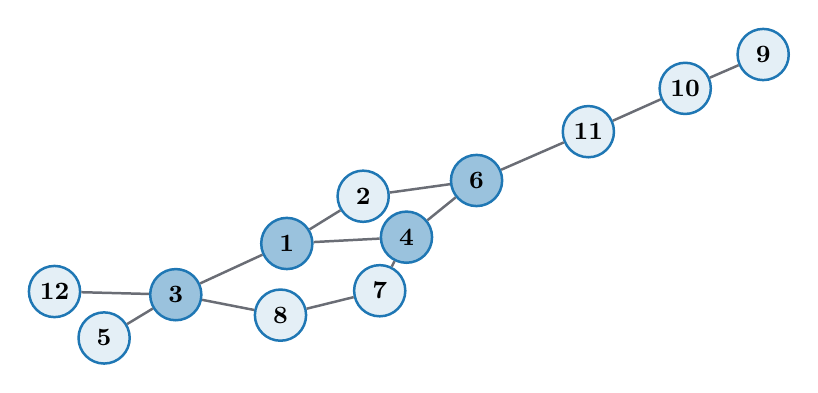
\begin{tikzpicture}[x=1.0cm, y=1.0cm]
  \node[gnode, ctr] (1)  at (2.95,1.20) {1};
  \node[gnode] (2)  at (3.92,1.80) {2};
  \node[gnode, ctr] (3)  at (1.54,0.55) {3};
  \node[gnode, ctr] (4)  at (4.47,1.28) {4};
  \node[gnode] (5)  at (0.63,0.00) {5};
  \node[gnode, ctr] (6)  at (5.36,2.00) {6};
  \node[gnode] (7)  at (4.13,0.60) {7};
  \node[gnode] (8)  at (2.87,0.29) {8};
  \node[gnode] (9)  at (9.00,3.60) {9};
  \node[gnode] (10) at (8.01,3.17) {10};
  \node[gnode] (11) at (6.78,2.62) {11};
  \node[gnode] (12) at (0.00,0.59) {12};
  \foreach \a/\b in {1/2, 1/3, 1/4, 2/6, 3/5, 3/8, 3/12, 4/6, 4/7, 6/11,
                     7/8, 9/10, 10/11}
    \draw[gedge] (\a) -- (\b);
\end{tikzpicture}
\end{center}

\vspace{-0.4em}
Edges: 1--2, 1--3, 1--4, 2--6, 3--5, 3--8, 3--12, 4--6, 4--7, 6--11, 7--8,
9--10, 10--11.

\begin{center}
\small
\renewcommand{\arraystretch}{1.15}
\begin{tabular}{|c|c|c|c|c|}
\hline
node & degree & $\sum_j d_{ij}$ (closeness) & betweenness & eigenvector ($\max = 1$) \\
\hline
1  & 3 & 25 (0.440) & 20 & \ans{1.000} \\ \hline
2  & 2 & 27 (0.407) &  8 & 0.705 \\ \hline
3  & \ans{4} & 28 (0.393) & 21 & 0.902 \\ \hline
4  & 3 & \ans{24} (\ans{0.458}) & 18 & 0.941 \\ \hline
5  & 1 & 38 (0.289) &  0 & 0.354 \\ \hline
6  & 3 & 26 (0.423) & \ans{25} & 0.796 \\ \hline
7  & 2 & 29 (0.379) &  5 & 0.601 \\ \hline
8  & 2 & 31 (0.355) &  3 & 0.590 \\ \hline
9  & 1 & 50 (0.220) &  0 & 0.070 \\ \hline
10 & 2 & 40 (0.275) & 10 & 0.177 \\ \hline
11 & 2 & 32 (0.344) & 18 & 0.382 \\ \hline
12 & 1 & 38 (0.289) &  0 & 0.354 \\ \hline
\end{tabular}
\end{center}

Centers: \ans{degree $=$ node 3} (4 against 3), \ans{closeness $=$ node 4}
(total distance 24 against 25), \ans{betweenness $=$ node 6} (25 against 21),
\ans{eigenvector $=$ node 1} (1.000 against 0.941). $\lambda_{\max} = 2.548$.
Four different nodes, each center unique.

\textbf{Marking.}

(a) [2] A connected, undirected graph, simple, with at most 12 nodes, drawn and
numbered. $-1$ if it is disconnected, or has a self-loop or a double edge, or
has 13 or more nodes (then (b) is marked on it as drawn). $0$ if nothing
checkable is drawn.

(b) [8] Two points for each measure: the center named \emph{and} the evidence
that it is the largest and that nothing ties with it. Mark each measure on the
student's own graph, not on the model graph.
\begin{itemize}[leftmargin=1.4em, itemsep=0.1em, topsep=0.2em]
  \item \emph{Degree.} Easy: the degrees are read off the drawing.
  \item \emph{Closeness.} The totals $\sum_j d_{ij}$ are integers, so a tie
        is a tie, exactly. Full marks need the top two totals shown. Closeness is
        large when the total is small, so the center is the node with the
        \emph{smallest} total. A student who picks the largest total has the
        measure upside down.
  \item \emph{Betweenness.} Credit counting by the definition: the shortest
        paths through the node, shared out when there are several. A fractional
        count such as $1/2$ for a pair with two routes is right.
  \item \emph{Eigenvector.} A student cannot solve $Ax = \lambda x$ for 12
        nodes by hand, and does not need to. Full marks: values from a few
        rounds of repeated multiplication by $A$ (start from all ones),
        or a stated check with code, that put the claimed center above
        the rest. Half marks: a plausible node with no numbers behind it.
        $0$: ``the node with the most links''. The model graph is built so that
        the eigenvector center (node 1, degree 3) is not the degree center
        (node 3, degree 4).
\end{itemize}
$-1$ from the total, once, if the four centers are not four different nodes but
each measure was argued correctly. That graph answers a different question.

\textbf{Traps in the task, so the marking is steady.}
\begin{itemize}[leftmargin=1.4em, itemsep=0.1em, topsep=0.2em]
  \item \emph{Ties.} A graph with a symmetric pair of nodes has two centers, not
        one. Krackhardt's kite (10 nodes) fails exactly this way: closeness is
        shared by two nodes, and degree and eigenvector pick the same node.
        A star or a path fails too: all four measures agree.
  \item \emph{Small graphs.} No graph with fewer than 10 nodes works. A student
        who claims one has a mistake in one of the four, usually closeness or
        eigenvector.
  \item \emph{Near ties in eigenvector.} Two nodes can differ by a few percent
        and the student's rounded numbers can hide it. Accept a claim that
        survives the student's own arithmetic; check hard ones with
        \texttt{check\_bcde.py}.
\end{itemize}

\textbf{How to check a student's graph.} Type its edge list into
\texttt{check\_bcde.py} (see README.md); it prints each center, whether it is
unique, and whether the four differ.

\end{document}
